\documentclass[document.tex]{subfiles}
\begin{document}

\chapter{Algorytm Viterbiego}
\section{Opis działania i zastosowania}
\indent Alogorytm Viterbiego został stworzony i przeanalizowany przez A.J. Viterbiego w 1967r. Jego zadaniem było dekodowanie kodów splotowych. Później odkryto że posiada cechy programowania dynamicznego i wykorzystuje maksymalne prawdopodobieństwo do określenia optymalnego zestawu tranzycji pomiędzy stanami. Algorytm został oryginalnie opracowany z myślą o zastosowaniach w telekomunikacji, ale znalazł zastosowanie w innych dziedzinach, m.in. w przetwarzanie obrazów, lokalizacji i rozpoznawaniu obiektów.\cite{viterbi_tutorial}
\\
\indent Główne zastosowanie algorytmu Viterbiego polega na
dekodowaniu informacji zakodowanych przy pomocy kodów splotowych. Sekwencja kodowana $m = m_1, m_2,...,m_n$, gdzie 
$m_i$ reprezentuje pojedynczy bit informacji, a indeks oznacza kolejność przesyłania. Enkoder splotowy przekształca informację wejściową w zakodowaną sekwencję $U = G(m)$.
Wykorzystuje do tego rejestr przesuwający, sumatory modulo-2 oraz wielomiany generujące(\textit{generator polynomials}) określające związek sumatorów z rejestrem.\cite{Comm_Sklar}\cite{viterbi_tutorial}

\begin{figure}[h]
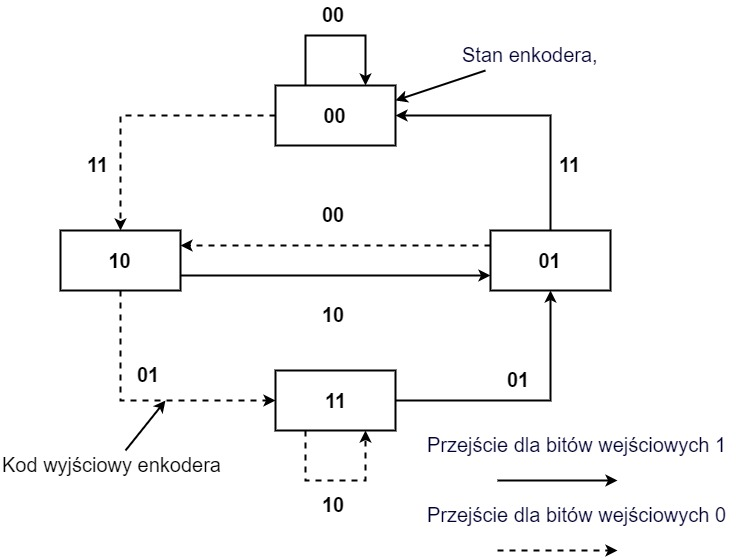
\includegraphics[scale=0.45]{conv_encoder}
\caption{Diagram stanów, dla enkodera o 3 bitowym rejestrze przesuwnym 
i dwóch sumatorach modulo-2 z wielomianami $g_1 = 111, g_2 = 101$ \protect\cite{Comm_Sklar}}
\label{fig:encoder}
\end{figure}

\clearpage
\indent Enkoder splotowy należy do klasy urządzeń zwanych automatami skończonymi(\textit{finite-state machines}), które zachowują informację o poprzednich sygnałach.
Jego działanie można zaprezentować w postaci diagramu stanów(\textit{state diagram}). Bieżący stan reprezentują pierwsze $K - 1$ bity rejestru o pojemności K, a przejścia pomiędzy stanami są określane przez kody wyjściowe.
Dla enkodera z 3 bitowym rejestrem przesuwającym i 2 bitowym wyjściem, stany są określone jako kolejno
$00, 01, 10, 11$. Diagram \ref{fig:encoder} przedstawia omawiany typ enkodera, ze wszystkimi możliwymi 
tranzycjami. Widoczne są dwa rodzaje przejść pomiędzy stanami - dla bitu wejściowego będącemu jedynką oraz dla zera. Do wizualizacji kolejnych tranzycji w czasie gdy ładowane są nowe dane do rejestru przesuwającego,
używane są diagramy kratowe(\textit{trellis diagram}).\cite{kody_splotowe}\cite{Comm_Sklar}\cite{viterbi_tutorial}
Kolumny diagramu oznaczają stany rejestru, wiersze kolejne momenty czasu $t_1, t_2, ..., t_n$. Linie łączące ze są węzły diagramu oznaczają tranzycje, które są wyzwalane pojawieniem się nowego bitu sygnału wejściowego w rejestrze enkodera(patrz rys. \ref{fig:encoder_trellis}).

\begin{figure}[h]
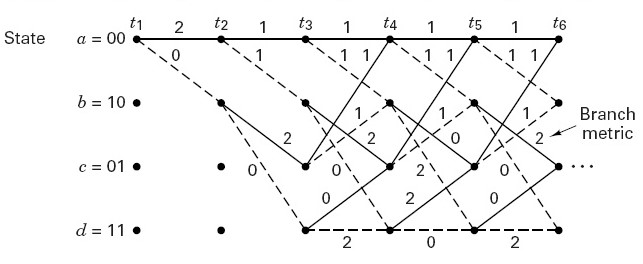
\includegraphics[scale=0.8]{encoder_trellis}
\caption{Diagram kratowy, dla enkodera o 3 bitowym rejestrze przesuwnym 
i dwóch sumatorach modulo-2 z wielomianami $g_1 = 111, g_2 = 101$ \protect\cite{Comm_Sklar}}
\label{fig:encoder_trellis}
\end{figure}

%5/31
\indent Po zakodowaniu informacji jest ona następnie poddawana modulacji - nałożenia wejściowego sygnału na analogowy sygnał nośny modulatora.\cite{Comm_Sklar}\cite{modulacja_put} Sygnał cyfrowy ze względu na małą częstotliwość jest podatny na zakłócenia w trakcie transferu. Stosując modulację 
sygnałem analogowym o wyższej częstotliwości możliwe jest przesyłanie informacji na większe odległości oraz zmniejszenie wpływu zakłóceń.
Sygnałem nośnym najczęściej są sygnały sinusoidalne, np. w postaci\cite{modulacja_agh_amp}\cite{modulacja_put}:

\begin{equation}
    f_c(t) = A_c cos(\omega t + \theta)
    \label{eq:module_carrier}
\end{equation}
\myequations{Funkcja sygnału nośnego modulatora\cite{modulacja_agh_amp}}

Na podstawie równania \ref{eq:module_carrier} można stwierdzić że występują trzy parametry, na które można wpłynąć do modyfikacji modulowanego sygnału - amplituda $A_c$, częstotliwość $\omega$ oraz faza $\theta$. Dlatego wyróżniamy trzy rodzaje modulacji(patrz rys.\ref{fig:modulation}):
\begin{itemize}
    \item modulacja częstotliwości - jest osiągana poprzez zmianę częstotliwości sygnału w zależności, czy w danym momencie występuje zmiana z 0 na 1(zwiększenie częstotliwości), czy z 1 na 0(zmniejszenie częstotliwości).
    \item modulacja amplitudy - polega na zmodyfikowaniu amplitudy sygnału nośnego przez amplitudę sygnału zakodowanego.
    \item modulacja fazy - różnica pomiędzy 0 i 1 w sygnale wejściowym jest reprezentowana przez zmianę startu sygnału sinusoidalnego nośnika, np. 0\degree dla 0 i 180\degree dla 1.
\end{itemize}
\clearpage
\begin{figure}[h]
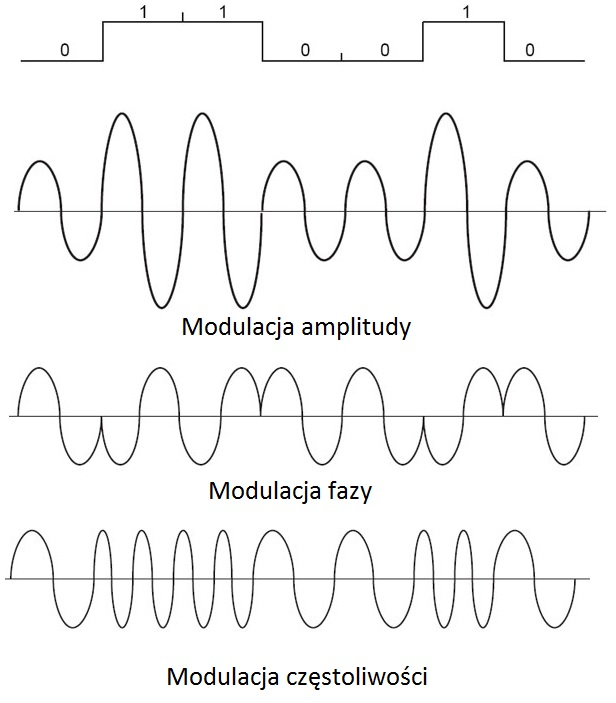
\includegraphics[scale=0.55]{modulation}
\caption{Rodzaje modulacji sygnału cyfrowego \protect\cite{Comm_Sklar}\cite{modulacja_put}}
\label{fig:modulation}
\end{figure} 

\indent Odbiornik dostaje zakodowaną, modulowaną i zakłóconą informację. W pierwszej fazie odczytywania przesłanego sygnału niezbędna jest jego demodulacja. Polega ona na odzyskaniu sygnału z wyjścia enkodera przed modulacją.
Dla sygnału modulowanego amplitudowo \textbf{AM} demodulacja może być przeprowadzona poprzez użycie detektora diodowego oraz filtracji niepożądanych wysokich częstotliwości.\cite{demodulation_am}
W przypadku demodulacji częstotliwościowej \textbf{FM} i fazy \textbf{PM}, wykorzystywane są detektory \textbf{PLL}(\textit{Phase Locked Loop} - pętla synchronizacji fazy)\cite{demodulation_fmpm}.

\begin{figure}[h]
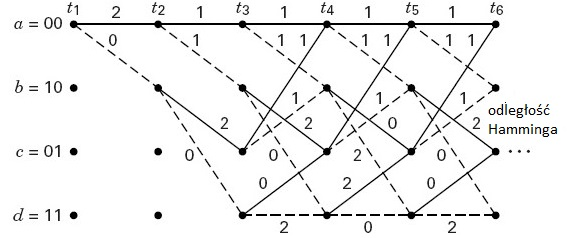
\includegraphics[scale=0.8]{viterbi_trellis}
\caption{Dekodowanie z wykorzystaniem algorytmu Viterbiego dla sekwencji zakodowanej enkoderem z 3 bitowym rejestrem przesuwnym i dwoma sumatorami modulo-2 o wielomianach $g_1 = 111, g_2 = 101$ \protect\cite{Comm_Sklar}}
\label{fig:viterbi_trellis}
\end{figure}

\indent W celu odczytania informacji zakodowanej enkoderem splotowym stosowany jest dekoder
wykorzystujący algorytm Viterbiego. Wykorzystuje on strukturę diagramu kratowego do obliczenia optymalnej
kombinacji przejścia pomiędzy jego stanami(patrz rys.\ref{fig:viterbi_trellis}). Do określenia najlepszego wariantu przejścia ze stanu w czasie $t_i$ do stanu $t_{i+1}$, wybierana jest tranzycja o najmniejszej odległości Hamminga\cite{Comm_Sklar} względem fragmentu kodu po demodulacji. Odległość Hamminga określana jest przez liczbę pozycji, na których różnią się dwa ciągi kodu.
Jeśli występuje kilka możliwych przejść do danego stanu, wybierane jest te, które ma największe prawdopodobieństwo - najmniejszą odległość Hamminga, a reszta jest odrzucana. Wybór najlepszego zestawu tranzycji
dla całego diagramu jest określony przez skumulowaną odległość Hamminga dla końcowego stanu. 
Na podstawie otrzymanej optymalnej listy przejść odczytywana jest zakodowana informacja .\cite{Comm_Sklar}\cite{viterbi_tutorial}\cite{viterbi_mit}
 %---------------------------------------------------------section end
 
\section{Wykrywanie linii na obrazie cyfrowym z wykorzystaniem algorytmu Viterbiego}\label{viterbi_line}
\indent Algorytm Viterbiego, którego celem jest znalezienie optymalnej ścieżki w diagramie kratowym, może zostać zastosowany w analogiczny sposób do wyznaczenia optymalnego zestawu współrzędnych pikseli na obrazie cyfrowym.
W tym wypadku piksele odpowiadają stanom rejestru przesuwającego, a odległość Hamminga wykorzystana do obliczenia najlepszej tranzycji jest zastąpiona funkcją intensywności pikseli. Zgodnie z zaproponowanym rozwiązaniem w \cite{viterbi_ch_9} dla każdego piksela określane jest najlepsze przejście do następnej kolumny/wiersza.

\begin{figure}[h]
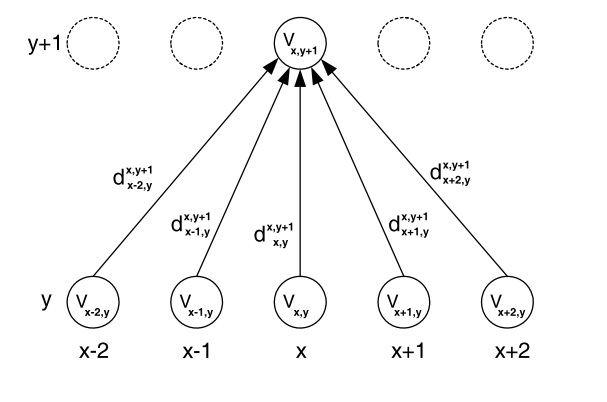
\includegraphics[scale=0.8]{viterbi_line_trellis}
\caption{Lokalne tranzycje diagramu kratowego dla obrazu cyfrowego\protect\cite{Mazurek_Robot_Viterbi}}
\label{fig:viterbi_trellis}
\end{figure}

Zakładając szukanie linii pionowej, przetwarzanie obrazu zaczyna się od pierwszego wiersza $y = 0$. 
Dla każdego z pikseli w pierwszym wierszu jest przypisana początkowa wartość akumulowana $V_{x, 0} = 0$
Dla piksela o współrzędnej $x, y$ rozpatrywana jest jego intensywność oraz intensywność jego sąsiadów.
Współrzędne sąsiednich pikseli są określane przedziałem $x + g$, gdzie $g\in \langle g_l;g_h\rangle$, np. $g_l = -2,\ g_h = 2$, czyli $g\in \{-2, -1, 0, 1, 2\}$. Wartość $V_{x,y+1}$ może być wyznaczana na podstawie równania \ref{eq:V}\cite{Mazurek_Robot_Viterbi}\cite{viterbi_ch_6}:

\begin{equation}
    V_{x, y+1} = max(V_{x+g, y} + d_{x+g, y}^{x,y+1}),\ g\in\{-2,-1,0,1,2\}
    \label{eq:V}
\end{equation}
\myequations{Równanie wyboru współrzędnej dla wykrywania linii wykorzystując algorytm
Viterbiego\cite{Mazurek_Robot_Viterbi}\cite{viterbi_ch_6}}


,gdzie $V_{x+g, y}$ - skumulowana dotychczasowa intensywność dla współrzędnych piksela ($x+g, y$), 
\\
$d_{x+g, y}^{x,y+1}$ - intensywność piksela o współrzędnych ($x+g, y$),  $V_{x, y+1}$ - wynikowa skumulowana intensywność dla piksela o współrzędnych (${x, y+1}$).
\\
Wartości $g$ określające najlepsze lokalną tranzycje są zapisywane w tablicy indeksów $L$ zgodnie z równaniem \ref{eq:L}\cite{Mazurek_Robot_Viterbi}\cite{viterbi_ch_6}:

\begin{equation}
   L_{y}^{x, y+1} = \argmax_{g}\limits(V_{x+g, y} + d_{x+g, y}^{x,y+1}),\ g\in\{-2,-1,0,1,2\}
    \label{eq:L}
\end{equation}
\myequations{Wyznaczanie tablicy indeksów dla algorytmu Viterbiego\cite{Mazurek_Robot_Viterbi}\cite{viterbi_ch_6}}

Indeksy są obliczane dla wszystkich rozpatrywanych wierszy. Po wyznaczeniu tablicy $L$ sprawdzany jest ostatni wiersz $y_max$ w celu określenia kolumny z największą skumulowaną intensywnością $x_max$ \ref{eq:xmax}:

\begin{equation}
   x_{y_{max}} = \max_{x}\limits(V_{x, y_max})
    \label{eq:xmax}
\end{equation}
\myequations{Określenie piksela z największą skumulowaną intensywnością dla ostatniej rozpatrywanej kolumny obrazu\cite{Mazurek_Robot_Viterbi}\cite{viterbi_ch_6}}

Wsteczne przetwarzanie tablicy indeksów $L$ pozwala wyznaczyć pozycję fragmentu linii dla pierwszej kolumny $y = 1$ \ref{eq:L_back}:

\begin{equation}
   x_{y-1} = x_y + L_{y-1}^{x,y},\ y = y_{max},...,y_{start + 1}
    \label{eq:L_back}
\end{equation}
\myequations{Określenie piksela z największą skumulowaną intensywnością dla ostatniej rozpatrywanej kolumny obrazu\cite{Mazurek_Robot_Viterbi}\cite{viterbi_ch_6}}

Do obliczenia wyników dla następnych kolumn zwiększa się $y_{start}$ i od nowa oblicza się tablice $V$ i $L$.
%-------------------end section----------------------------------------

\section{Implementacja detekcji linii języku C++}
\indent Tworząc aplikację wykorzystującą algorytm Viterbiego do lokalizacji linii
na obrazie cyfrowym skorzystano z nowych funkcjonalności standardu C++11. 
Zdjęcia na, których szukano linii były wczytywane używając funkcji biblioteki
\code{CImg}\cite{cimg_doc}. Reprezentowane przez obiekty \code{Cimg<T>}, dane pikseli zdjęcia były kopiowane do
dynamicznie zaalokowanych tablic przypisanych do obiektów \code{std::unique\_ptr}. Skorzystano inteligentnego wskaźnika \code{std::unique\_ptr} , ze względu na funkcję automatycznego zwalniania zaalokowanych zasobów po wywołaniu jego destruktora\code{std::unique\_ptr}.  
Wszystkie warianty implementacji detekcji linii zostały zawarte w klasie \code{Viterbi}, 
jako jej metody. 

%opis listinigu opencl_viterbi.cpp
\subsection{Wersja szeregowa}
\indent Pierwsza podstawowa implementacja algorytmu detekcji linii, w wykonuje wszystkie operacje w sposób sekwencyjny  w ramach tego samego wątku. Została stworzona jako punkt odniesienia szybkości wykonania względem później omawianych algorytmów współbieżnych.
\\
\indent Wersja szeregowa algorytmu Viterbiego do detekcji linii jest metodą klasy \code{Viterbi} o nazwie
\\ \code{viterbiLineDetect}. Przyjmuje trzy argumenty wejściowe:
\begin{enumerate}
    \item \code{std::vector<unsigned int> \&line\_x} - referencja kontenera, do którego zapisywane są współrzędne szukanej linii
    \item \code{int g\_low} i code{int g\_high} : określają zakres rozpatrywanego sąsiedztwa każdego piksela przy
    wyznaczaniu macierz V(patrz równanie \ref{eq:V})
\end{enumerate}
Informacje o intensywności pikseli obrazu pobierane są używając składowej \code{const unsigned char *m\_img}.
\clearpage
Kod we wnętrzu funkcji dzieli się na:
\begin{enumerate}
    \item Inicjalizację(patrz rys. \ref{lst:viterbi_serial_init})
    \item Pętlę przejścia przez wszystkie kolumny obrazu, w której dla każdej z nich wykonywane są kroki przedstawione we wzorach \ref{eq:V} do \ref{eq:L_back}.(patrz rys. \ref{lst:viterbi_serial_loop})
\end{enumerate}

\lstinputlisting[language={C++}, label={lst:viterbi_serial_init}, caption=Inicjalizacja zmiennych, linerange=219-233, firstnumber=219]{viterbi_source/Viterbi.cpp} 

\lstinputlisting[language={C++}, label={lst:viterbi_serial_loop}, caption=Główna pętla programu, linerange=234-290, firstnumber=234]{viterbi_source/Viterbi.cpp} 

\begin{figure}[h]
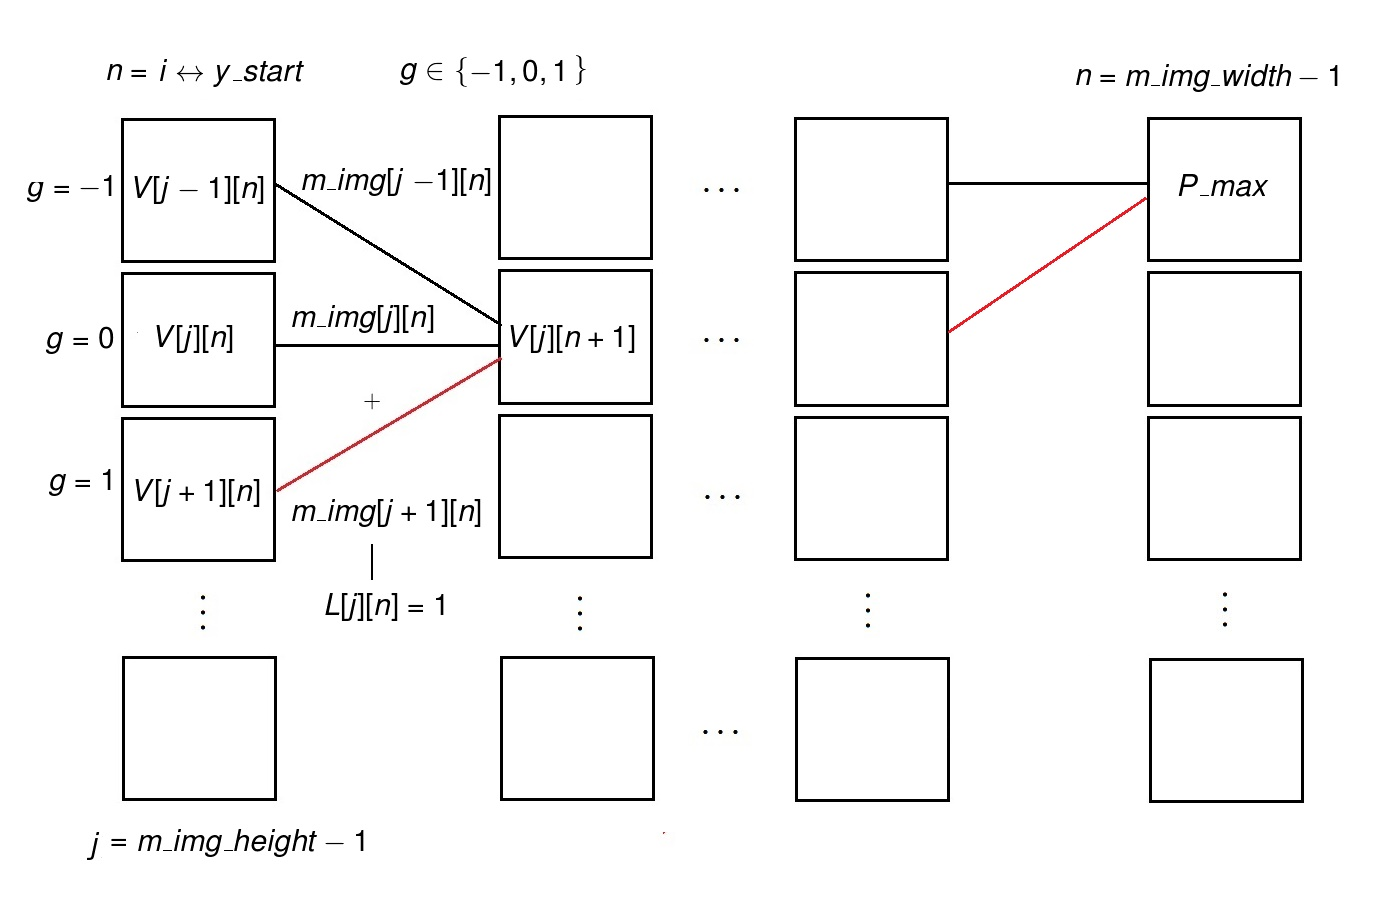
\includegraphics[scale=0.45]{viterbi_serial_nodes}
\caption{Schemat działania algorytmu szeregowego}
\label{fig:viterbi_serial_nodes}
\end{figure}

%-------------end subsection--------------------
\clearpage
%opisać wszystkie fragmenty z odniesieniem do schematu ogólnego algorytmu - shcemat z atykułów i wzory
\subsection{Wersja równoległa - C++11}
%opisać wykorzystanie obiektów std future odniesc do rozdzialu 2 i opisac jak dzielona jest praca
%wrzucic rysunek jak to działa
\indent Na podstawie wcześniej przedstawionego algorytmu detekcji linii oraz opisanej szeregowej implementacji można stwierdzić, że możliwe jest oddzielne przetwarzanie kodu dla każdej z kolumn reprezentowanych licznikiem
\code{i} pętli z listingu \ref{lst:viterbi_serial_loop}. Pierwszym z wariantów, który wykorzystuje 
podaną cechę algorytmu jest implementacja wielowątkowa. Korzysta ona z funkcji i obiektów nagłówka \code{<thread>}, w tym wypadku używany jest obiekt \code{std::future} do przechowywania rezultatów wykonania
wątków. Ponadto do uruchamiania nowych wątków stosowana jest funkcja \code{std::async()}, która uruchamia dodatkowe wątki(patrz rozdział 3.2.3).
%listing uruchomianie wątków - poprawić formatowanie - załamac linie 405
\lstinputlisting[language={C++}, label={lst:viterbi_threads}, caption=Wielowątkowa implementacja algorytmu detekcji linii, linerange=383-418, firstnumber=383]{viterbi_source/Viterbi.cpp} 

\indent W celu właściwego wykorzystania zasobów procesora stosowana jest funkcja \code{std::thread::hardware\_concurrency()} do określenia rekomendowanej liczby jednocześnie uruchomionych wątków.
Cały obraz jest przetwarzany fragmentami po \code{num\_of\_threads} wątków na raz, gdzie dla każdego z nich przypisana jest inna kolumna startowa $y_{start}$(patrz równanie \ref{eq:L_back}). 
Funkcja wykonywana przez wątki jest bardzo podobna jak dla wersji szeregowej(patrz listingi \ref{lst:viterbi_serial_loop} i \ref{lst:viterbi_serial_init}). Różni się brakiem głównej pętli - nie jest potrzebna iteracja po wszystkich możliwych $y_{start}$, rozpatrywana jest tylko kolumna odpowiadająca zmiennej \code{start\_col} z listingu \ref{lst:viterbi_threads}. Ponadto nie jest przekazywana referencja do wektora \code{line\_x} tylko wynik jest zwracany przez wątek i zapisywany w \code{line\_x} przez funkcję tworzącą wątki(\code{launchViterbiMultiThread}). 
\clearpage
\indent Po tym jak wszystkie wątki wykonają swoje obliczenia wynik jest zapisywany i zaczyna się nowa iteracja, w której rozpatrywany jest następny zestaw kolumn obrazu. Pętla będzie się wykonywać dopóki nie zostaną przetworzone wszystkie kolumny, co reprezentowane jest przez wartość licznika \code{to\_process}(patrz rys.\ref{fig:threads_viterbi}).

\begin{figure}[h]
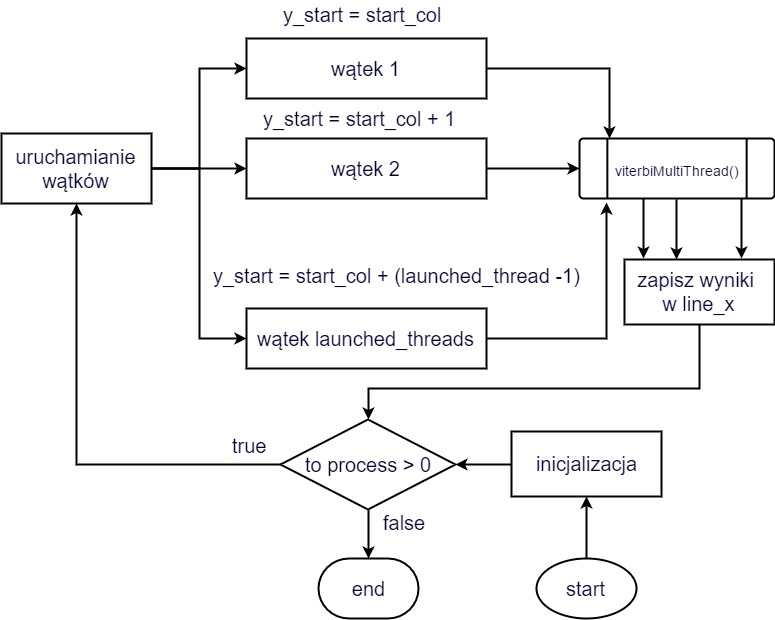
\includegraphics[scale=0.7]{threads_viterbi}
\caption{Schemat działania algorytmu szeregowego}
\label{fig:threads_viterbi}
\end{figure}

\clearpage
\subsection{Wersja równoległa - wykorzystanie biblioteki OpenCL}
\indent Podobnie jak dla wersji wielowątkowej algorytm wykrywania linii został zmodyfikowany,tak aby 
zrównoleglić główną pętlę listingu \ref{lst:viterbi_serial_loop} : $y_{start} = 0,1,.., y_{n-1}$.
Założono, że dla stworzonej przestrzeni indeksowej OpenCL, każda kolumna startowa odpowiada elementowi roboczemu(\textit{work-item}). 
\indent Pamięć globalna GPU jest zdecydowanie większa od lokalnej, osobnej dla każdej grupy roboczej.
Z tego powodu zdecydowano się na zdefiniowanie buforów zaalokowanych w pamięci globalnej karty graficznej.
Wynika to z faktu możliwości przetwarzanie zdjęć o dużej rozdzielczości. Każda karta graficzna posiada różną wielkość dostępnej pamięci globalnej i lokalnej, dlatego w metodzie \code{viterbiLineOpenCL\_cols} odpowiedzialnej za detekcję linii użyto funkcji OpenCL do sprawdzenia dostępnej pamięci globalnej oraz maksymalnego rozmiaru bufora.(patrz funkcja \code{clGetDeviceInfo} z listingu \ref{lst:opencl_memcheck}). Jeśli okaże się, że
utworzenie jednego z buforów przekracza limit dostępnej pamięci, wtedy obraz jest przetwarzany w fragmentach
określanych wielkością \code{global\_size} obliczaną w linijkach 324 - 328 listingu \ref{lst:opencl_memcheck}.

%memory check
\lstinputlisting[language={C++}, label={lst:opencl_memcheck}, caption=Sprawdzanie dostępnej pamięci karty 
graficznej, linerange=303-324, firstnumber=303]{viterbi_source/Viterbi.cpp} 

\indent Dla zbudowanego kernela zdefiniowano bufory(patrz listing \ref{lst:opencl_buffers}):
\begin{itemize}
\item \code{cmImg} : bufor do odczytu danych pikseli zdjęcia
\item \code{cmLine\_x} : bufor do zapisu obliczonych współrzędnych linii
\item \code{cmV1}, \code{cmV2} : bufory emulujące macierz skumulowanej intensywności $V$
\item \code{cmL} : trójwymiarowy bufor składający się z \code{global\_size} macierzy indeksów $L$
\end{itemize}
Bufory \code{V1} i \code{V2} zostały stworzone w celu zminimalizowania wykorzystania pamięci karty graficznej.
Zamiast użycia całej macierzy V, rozpatrywane są tylko dwie kolumny - obecna i następna. Kolumna
\code{V1} jest inicjalizowana zerami(patrz rozdział \ref{viterbi_line}), następnie wyniki dla poszczególnych 
wierszy są zapisywane w \code{V2}. W następnej iteracji w kolumnie \code{V1} są zapisywane wyniki na podstawie rezultatów poprzedniej iteracji zapisanych w \code{V2}. W analogiczny sposób przetwarzane są pozostałe kolumny z zakresu $\langle$\code{start\_column} ; \code{global\_size}$\rangle$.

%create buffers
\lstinputlisting[language={C++}, label={lst:opencl_buffers}, caption=Tworzenie buforów wymiany danych i ustawienie
argumentów kernela, linerange=326-344, firstnumber=326]{viterbi_source/Viterbi.cpp} 

%opis kernela - dodać rysunki buforów L i V1, V2 z naniesionymi zmiennymi kernela
\indent Oprócz stworzonych buforów, jako argumenty do kernela podawane są szerokość, wysokość zdjęcia oraz 
zakres lokalnie rozpatrywanych wierszy \code{g} $\in \langle$\code{g\_low}; \code{g\_high} $\rangle$.
Wnętrze kodu kernela (patrz listing \ref{lst:opencl_kernel}) jest bardzo podobne do wersji szeregowej
dla CPU, ale tak jak dla wersji wielowątkowej wyeliminowana jest główna pętla przetwarzająca wszystkie
$y_{start}$(patrz rozdział \ref{viterbi_line}). Każde $y_{start}$ odpowiada globalnemu id poszczególnego
elementu roboczego, otrzymanego po wywołaniu funkcji \code{get\_global\_id}.
Każdemu elementowi roboczemu odpowiada fragment trójwymiarowego bufora \code{L} określany przez zmienną
\code{L\_id}, otrzymany na podstawie wyznaczonej kolumny startowej. Dodatkowo decyduje ona
o numerze kolumny dla zmiennych \code{V1} i \code{V2}. Ostatnim wyróżniającym fragmentem kodu jest zapisanie
pozycji piksela z największą skumulowaną intensywnością - \code{x\_n}. Indeks bufora \code{line\_x} nie jest
decydowany tylko przez wyznaczony numer kolumny startowej, ale również na podstawie przyjętego argumentu
\code{first\_col}.

%kernel opencl
\lstinputlisting[language={C}, label={lst:opencl_kernel}, caption=Kernel do detekcji linii, linerange=1-76, firstnumber=1]{viterbi_source/viterbi_kernel.cl} 

%dodać zdjęcia buforów i będzie stykać

\indent Parametr \code{first\_col} jest wyznaczany na podstawie wielkości przetwarzanego zdjęcia,
na początku ma wartość 0, ale w kolejnych iteracjach pętli z listingu \ref{lst:opencl_detect},
zwiększany jest o rozmiar \code{global\_size}, aż będzie równy szerokości zdjęcia \code{m\_img\_width}.
Wyniki po wykonaniu kernela przez wszystkie elementy robocze są odczytywane z bufora \code{cmLine\_x} i 
kopiowane do kontenera \code{line\_x} używając funkcji \code{clEnqueueReadBuffer}(patrz linijka 360 z listingu
\ref{lst:opencl_detect})

%read results
\lstinputlisting[language={C++}, label={lst:opencl_detect}, caption=Wyznaczenie współrzędnych linii, linerange=352-364, firstnumber=352]{viterbi_source/Viterbi.cpp} 


%-------!!!!!!!!!!!!!!!!!!!!!!!!!!!!!!!!!!!!!---------
%
%   Popraw rysunek dla C++11 - przy bloku warunkowym dodaj T/N do strzałek
%
%--------!!!!!!!!!!!!!!!!!!!!!!!!!!!!!!!!!!!!!---------

\end{document}